\documentclass{article}
\usepackage{CJKutf8}
\usepackage{multirow}
\usepackage{listings}
\usepackage{graphicx}
\usepackage{subfigure}
\begin{CJK}{UTF8}{gbsn}
\usepackage[framed,numbered,autolinebreaks]{mcode}
\begin{document}
\title{通信系统第三次作业}
\author{王亭午, 无210班, 2012011018}
\date{2015年5月30号}
\maketitle
\section{作业一}
多径信道和时域判决反馈均衡器的仿真练习。随机产生长为10000bit的01序列,采用
QPSK调制,格雷码映射。信道模型为(1)直射信道 h=1; (2)多径信道,强度 h\_dB \(=[0,-6,-8,-10]\)(单位为 dB);
对应的时延 h\_time \(=[0,2,5,16]\)(单位为符号周期);
假设接收机处的信噪比SNR=15dB。
\subsection*{a. 时域冲激响应}给出信道(2)的时域冲激响应图\\
代码在main.m中,逻辑比较简单,不在这里列出来。效果图Fig. 1,Fig. 1下半图为对数坐标小的图。
\begin{figure}[b!]
\centering
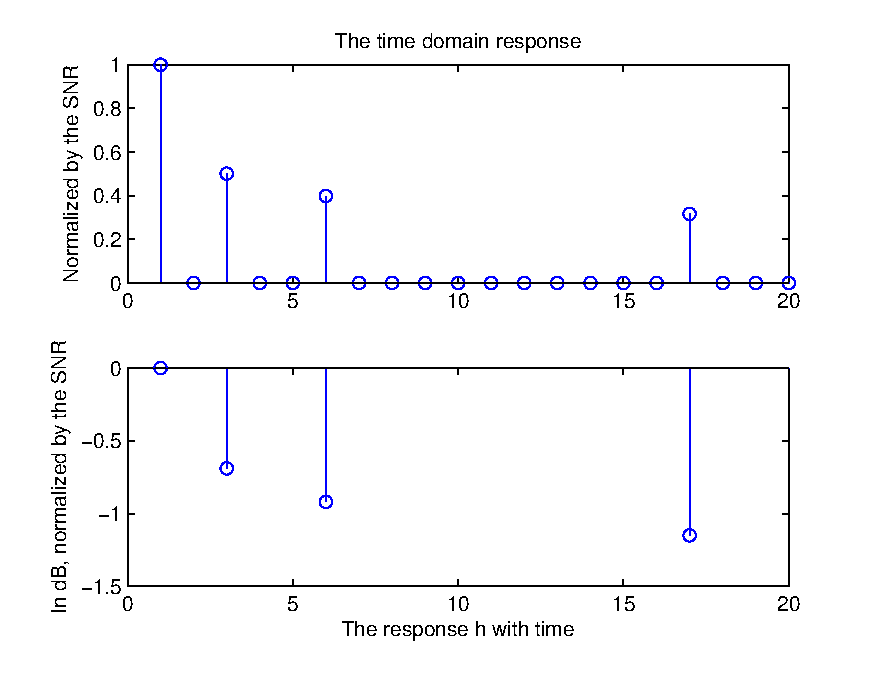
\includegraphics[width=9cm]{1.eps}
\caption{}
\end{figure}
\subsection*{b. 星座图}分别给出序列经过信道前后的星座图\\
可以看到,在通过我们的信道之后,星座图出现了非常大的变化。原图中的信号全部集中在4个qpsk传输点上。
而在接收端,大量的接受的qpsk信号都偏离了原来的位置,信号之间互相干扰。
值得注意的是,接受信号存在明显的模式(pattern),这为之后的滤波提供了可能。
\begin{figure}[h]
\begin{minipage}[t]{0.5\linewidth}
\centering
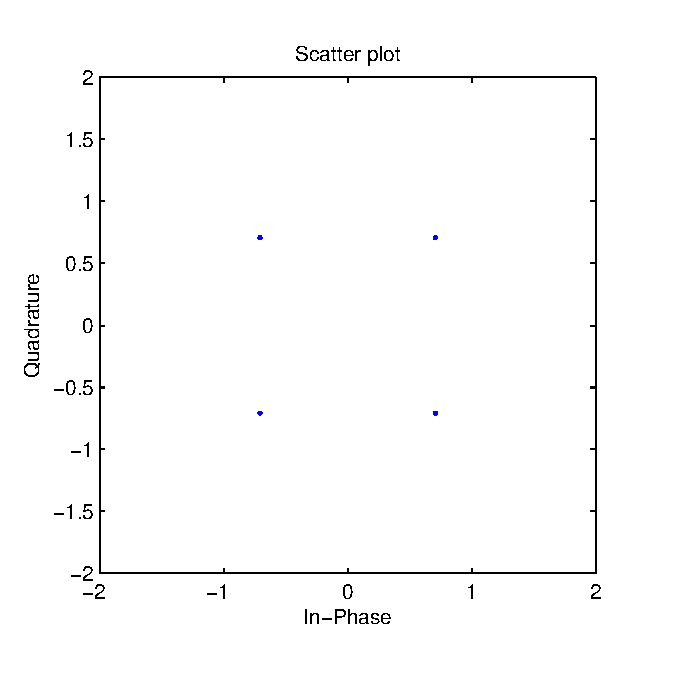
\includegraphics[width=2.2in]{2.eps}
\caption{输入前星座图}
\label{fig:side:a}
\end{minipage}%
\begin{minipage}[t]{0.5\linewidth}
\centering
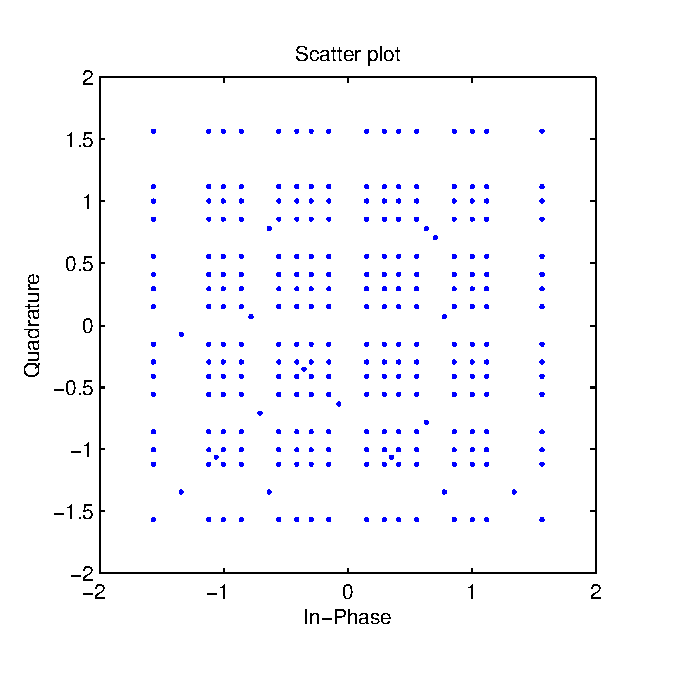
\includegraphics[width=2.2in]{3.eps}
\caption{输入后星座图}
\label{fig:side:b}
\end{minipage}
\end{figure}
\subsection*{c. LMS}假设已知该序列的前500个点,作为训练序列。采用时域的判决反
馈均衡器进行均衡,采用LMS准则,均衡器的抽头数量为32。给出训练过程中的误差曲线和未知序列经过均衡处理后的星座图。\\
代码为main2.m,迭代参数的代码如下:
值得注意的是,迭代的初始点非常的重要。在实际情况中,我们选取\(W_1\)最大,
因为我们知道直射信道依然是最好的信道。如果初始点选择错误,很有可能会发生发散性震荡。
在迭代中,我使用了归一化LMS算法,\(c_0 = 0.01,\,\mu = 0.001\)。
\begin{equation}
\mu' = \frac{\mu}{c_0 + \frac{1}{L}\sum\nolimits|x_k|^2}
\end{equation}
\begin{lstlisting}
function weight = LMS(raw_output, true_output, nWeight)
% raw_output -> x, true_output -> y, y_i = \sum(xTw)

% initialize the weight factor
weight = zeros(nWeight, 1);
weight(nWeight) = 1;

mu = 0.001;
c0 = 0.01;
mu_unified = mu / (c0 + sum(raw_output' * raw_output) ...
    / nWeight);
% append nWeight zeros to enable the calculations
raw_output = [zeros(nWeight - 1, 1); raw_output];
% loop until convergence
lastTimeError = 0;
while 1
    % renew the raw output
    predict_output = zeros(length(true_output), 1);
    for iWeight = 1: 1: nWeight
        predict_output = predict_output + weight(iWeight) * raw_output(iWeight: length(true_output) + iWeight - 1);
    end
    
    % get the error of the target function
    target_error = true_output - predict_output;
    
    % break if stoped
    if abs(sum(target_error' * target_error) - lastTimeError) < 0.01
        break
    end
    
    lastTimeError = sum(target_error' * target_error);
    %fprintf('The overall error is now %f\n', lastTimeError);
    
    for iWeight = 1: 1: nWeight
        % get the unifying descedent steps and decent
        descent = target_error' * raw_output(iWeight: length(true_output) + iWeight - 1);
        weight(iWeight) = weight(iWeight) + 2 * mu_unified * descent;
    end
end
\end{lstlisting}
\begin{figure}[h]
\begin{minipage}[t]{0.5\linewidth}
\centering
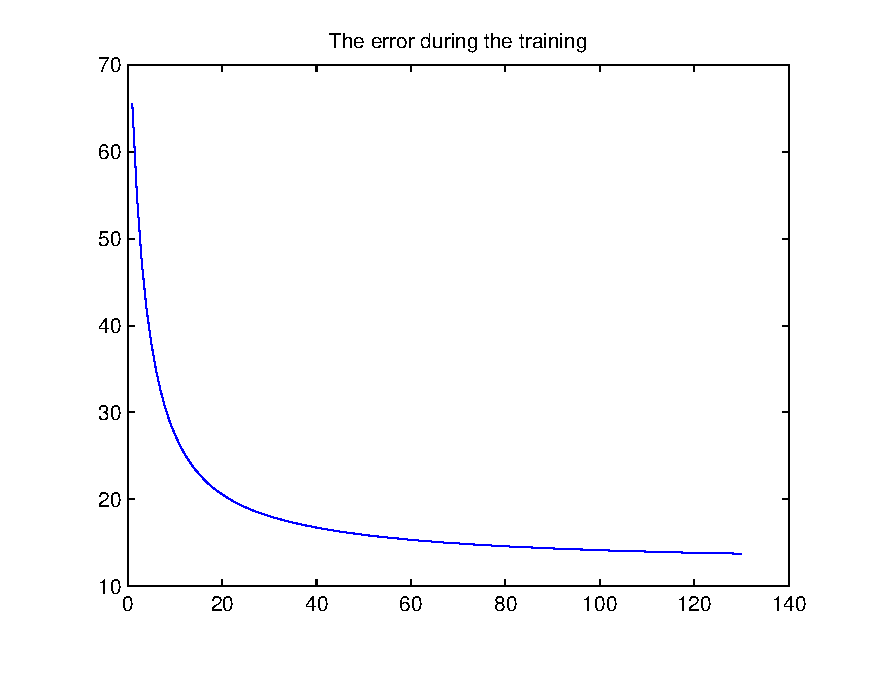
\includegraphics[width=2.2in]{4.eps}
\caption{训练中误差曲线}
\label{fig:side:a}
\end{minipage}%
\begin{minipage}[t]{0.5\linewidth}
\centering
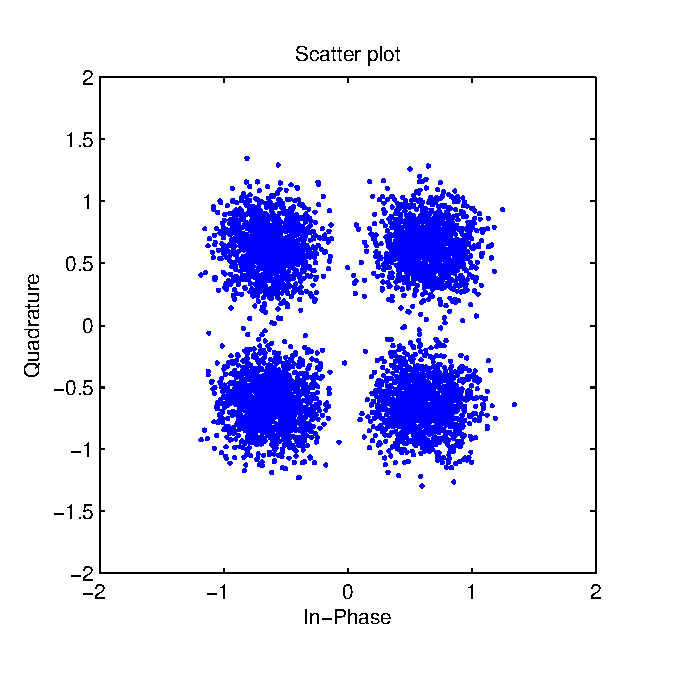
\includegraphics[width=2.2in]{5.eps}
\caption{均衡化后星座图}
\label{fig:side:b}
\end{minipage}
\end{figure}
可以看到,均衡化后,原本的四个qpsk点被恢复,效果非常明显。
\subsection*{d. BER曲线}
取信噪比 SNR=[0:15]dB,给出c)中未知序列经过均衡处理后的误码率(BER)曲线。
注意,纵坐标请用对数坐标表示。与AWGN信道下QPSK调制的标准BER曲线对比。\\
代码在main2.m,使用一个简单的平坦分部噪音来模拟噪声。效果图如下:
\begin{figure}[h]
\begin{minipage}[t]{0.32\linewidth}
\centering
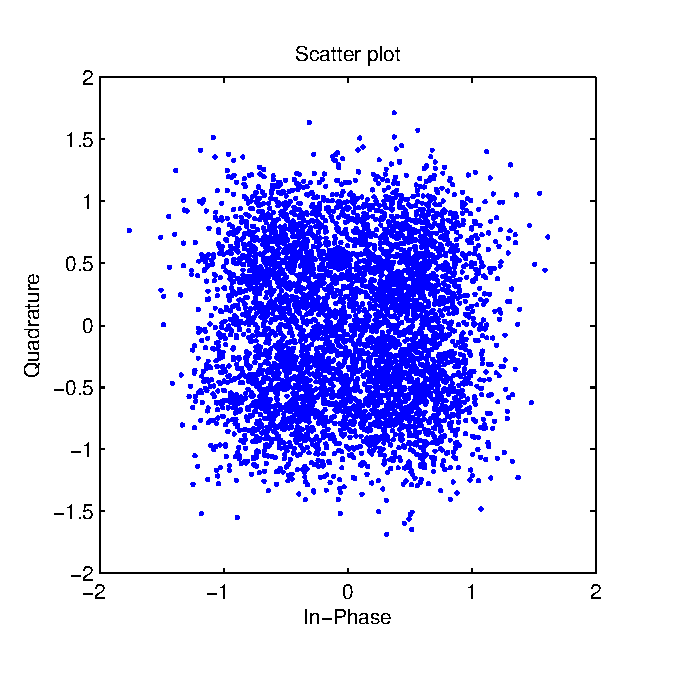
\includegraphics[width=1.2in]{61.eps}
\end{minipage}%
\begin{minipage}[t]{0.32\linewidth}
\centering
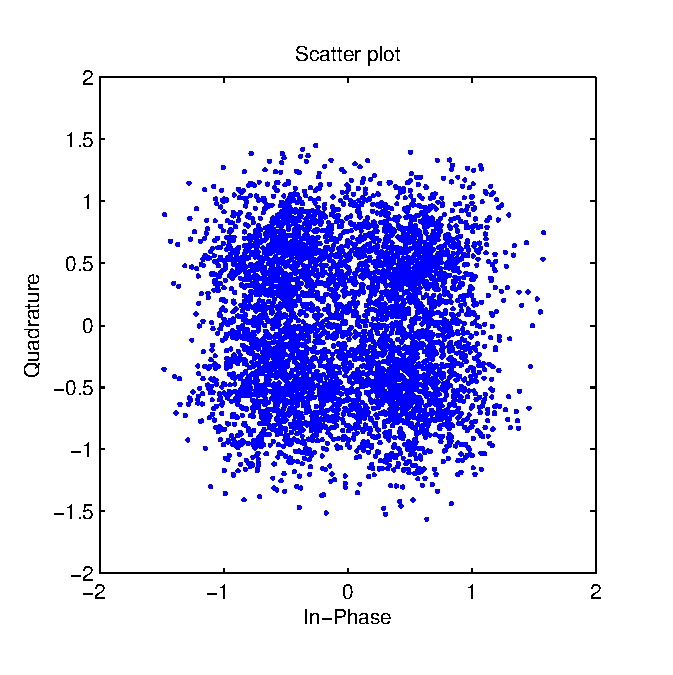
\includegraphics[width=1.2in]{62.eps}
\end{minipage}%
\begin{minipage}[t]{0.32\linewidth}
\centering
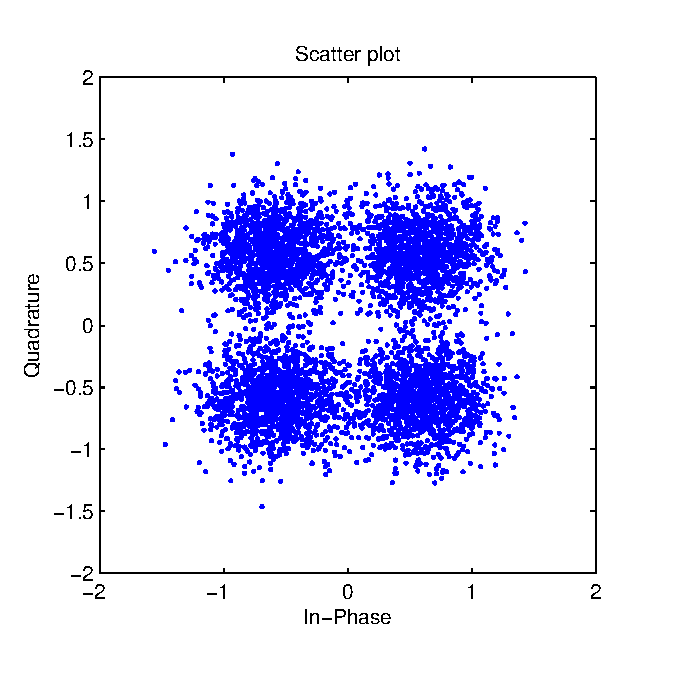
\includegraphics[width=1.2in]{65.eps}
\end{minipage}%
\end{figure}
\begin{figure}[h]
\begin{minipage}[t]{0.32\linewidth}
\centering
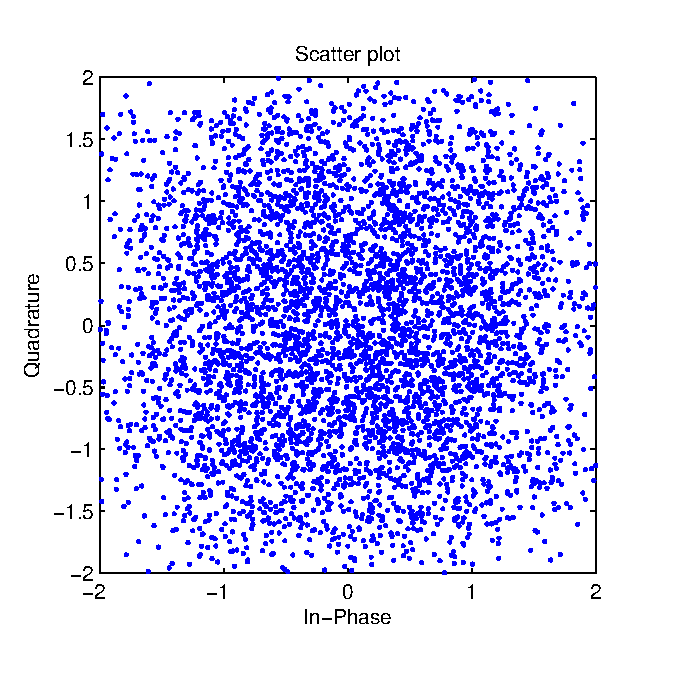
\includegraphics[width=1.2in]{71.eps}
\end{minipage}%
\begin{minipage}[t]{0.32\linewidth}
\centering
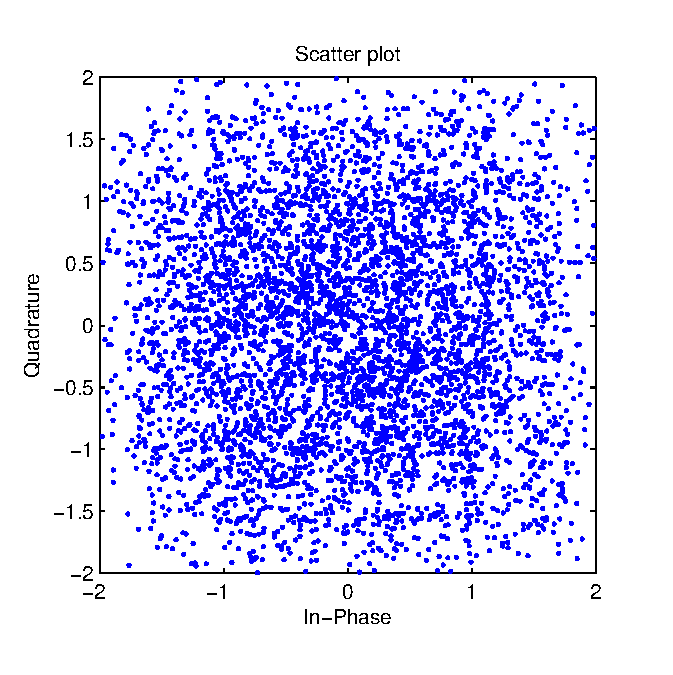
\includegraphics[width=1.2in]{72.eps}
\end{minipage}%
\begin{minipage}[t]{0.32\linewidth}
\centering
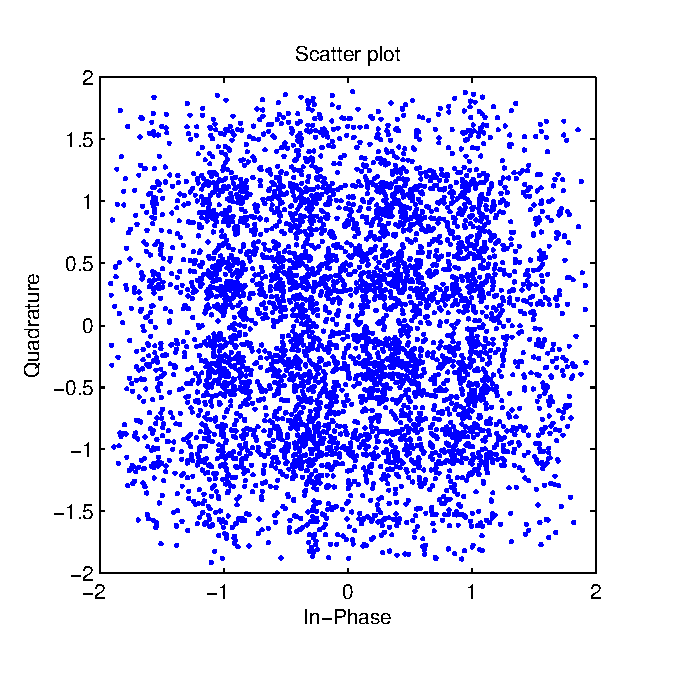
\includegraphics[width=1.2in]{75.eps}
\end{minipage}%
\end{figure}
\begin{figure}[h!]
\centering
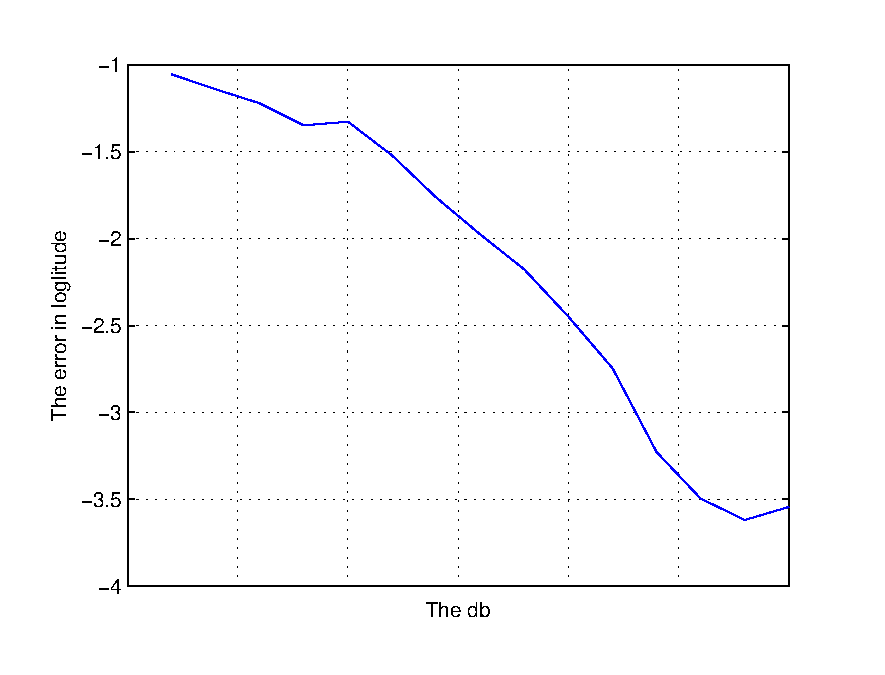
\includegraphics[width=9cm]{8.eps}
\caption{BER误差曲线}
\end{figure}
\subsection*{e. Blind LMS}
 (选做)在某些特定场景下,我们无法知道训练序列,或者为了提高传输效率而不
采用训练序列。此时可以采用盲均衡技术对接收信号进行处理。请调研一种针对
QPSK的盲均衡算法,并重复c)和d)中的仿真。\\
这里采用一个简单的oversample的方法来解决Blind LMS的问题。
我们使用的论文是[1]中的方法。通过过采样,我们将每一个数据发送多个copy。对数据进行交织编码,打乱顺序,从而减少信道影响。\\
\noindent [1] {Watanabe, K. and Komatsu, M. and Matsumoto, H. and Furukawa, T.}, 2013.\ \lq \lq A proposal of blind equalization algorithm using over-sampling for received signals including noise. \rq \rq\ \emph{Intelligent Signal Processing and Communications Systems (ISPACS), 2013 International Symposium on}\\
可以从图7中看到,这个算法是非常有效的。不过代价是传输了重复的信息来增加准确度。
\begin{figure}[t!]
\centering
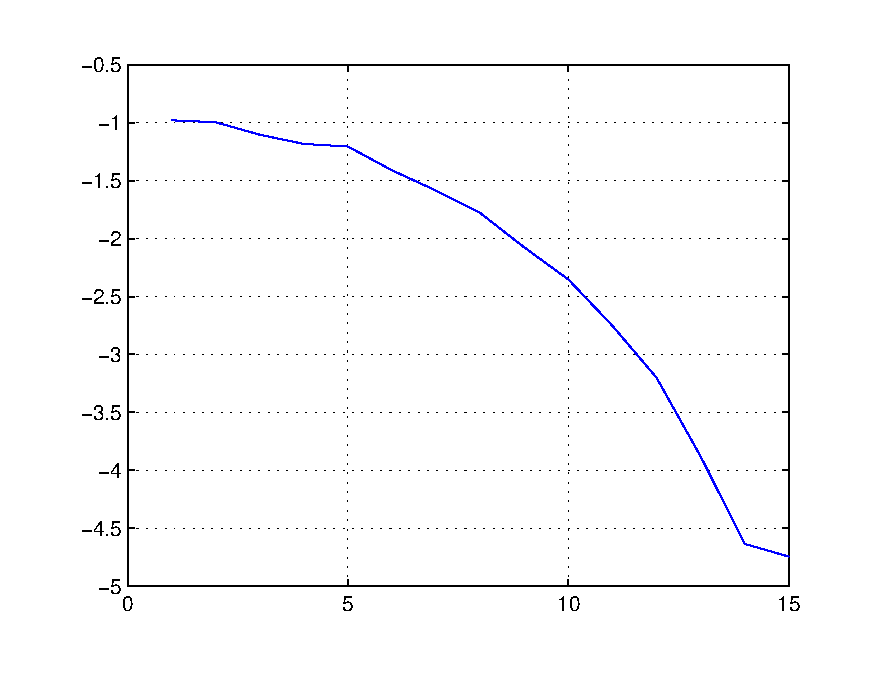
\includegraphics[width=9cm]{9.eps}
\caption{该算法BER曲线}
\end{figure}
\section{作业二}
当测量小尺度传播时,假设连续采样值在时间上有很强的相关性,需要确定合适的空间采样间隔。
假设某信号的载频为f=2700MHz,移动速率为v=35m/s,求该信号的多普勒频移\(f_m\)是多少?
再假设能够在运动的车辆上实时地进行测量,请问移动20m需要多少采样值?
(若相干时间定义为相干函数大于0.5时的时间,则相干时间可近似为:\(T_C = 9/(16\pi f_m)\))

\end{CJK}
\end{document}